\section{Fast poisson logpmf}
\subsection{The implementations}
The poisson logpmf is something aaaa

We have four different implementations performing (poisson logpmf?) ... :


\definecolor{keywordclr}{rgb}{0,0,1}
\definecolor{stringclr}{rgb}{0.75,0.15,0.15}
\definecolor{commentclr}{rgb}{0.5,0.5,0.5}

\lstset{frame=tb,
  language=Python,
  aboveskip=3mm,
  belowskip=3mm,
  showstringspaces=false,
  columns=flexible,
  basicstyle={\small\ttfamily},
  numbers=left,
  numberstyle=\smaller\color{commentclr},
  keywordstyle=\color{keywordclr},
  commentstyle=\color{commentclr},
  stringstyle=\color{stringclr},
  breaklines=true,
  breakatwhitespace=true,
  tabsize=4
}

The first implementation we consider is the implementation provided by the SciPy \cite{SciPy}.
This implementation runs on the CPU.
\begin{lstlisting}
from scipy.stats import poisson

def poisson_logpmf(k, r):
    return poisson.logpmf(k, r)
\end{lstlisting}

The second implementation is an implementation created by I\&K using NumPy \cite{NumPy} and SciPy.
This implementation also runs on the CPU, but is nearly twice as fast as the one provided by the SciPy library when the k and r matrices have 40 million elements each.
\begin{lstlisting}
import numpy as np
import scipy

def poisson_logpmf(k, r):
    return k * np.log(r) - r - scipy.special.gammaln(k+1)
\end{lstlisting}

The third implementation piggybacks off of the previous NumPy implementation, but is ported to CuPy \cite{CuPy}.
This implementation achieves large speed increases over the NumPy equivalent for large matrices.
\begin{lstlisting}
import cupy as cp 

def poisson_logpmf(k, r):
    return k * cp.log(r) - r - cupyx.scipy.special.gammaln(k+1)
\end{lstlisting}

\lstset{frame=tb,
  language=C++,
  aboveskip=3mm,
  belowskip=3mm,
  showstringspaces=false,
  columns=flexible,
  basicstyle={\small\ttfamily},
  numbers=left,
  numberstyle=\smaller\color{commentclr},
  keywordstyle=\color{keywordclr},
  commentstyle=\color{commentclr},
  stringstyle=\color{stringclr},
  breaklines=true,
  breakatwhitespace=true,
  tabsize=4
}

The CUDA implementation (just the kernel).
\begin{lstlisting}
__global__ void poisson_logpmf_kernel(const int *k, const float *r, float *out)
{
  int i = blockIdx.x * blockDim.x + threadIdx.x;
  out[i] = k[i] * logf(r[i]) - r[i] - lgammaf(k[i]+1);
}
\end{lstlisting}


Both the CuPy and the CUDA implementations allow for all, some or none of the input matrices to be located in the GPU's global memory. 
Any input not located in GPU memory will be copied to the device in order for the computation to be performed by the GPU.
Only when both inputs are located on the host will the returned results also be located on the host, meaning that the input matrices will be copied from the host to the device for computation, before the result is copied from the device back to host.
This introduces some extra variations for the CuPy and CUDA implementations, resulting in the following set of variations for both of them:
\begin{compactitem}
  \item
    When both of the input matrices are located on the host, and the returning data is located on the host: hh2h
  \item
    When one of the input matrices are located on the host and the other on the device, and the returning data is located on the device: dh2d
  \item
    When both of the input matrices are located on the device, and the returning data is located on the device: dd2d
\end{compactitem}
We omit the variation where both the inputs are located on the host and the output is located on the device.

\begin{figure}[ht!]\label{figure:poisson_logpmf_performance}
\hspace*{3cm}
%\begin{center}
  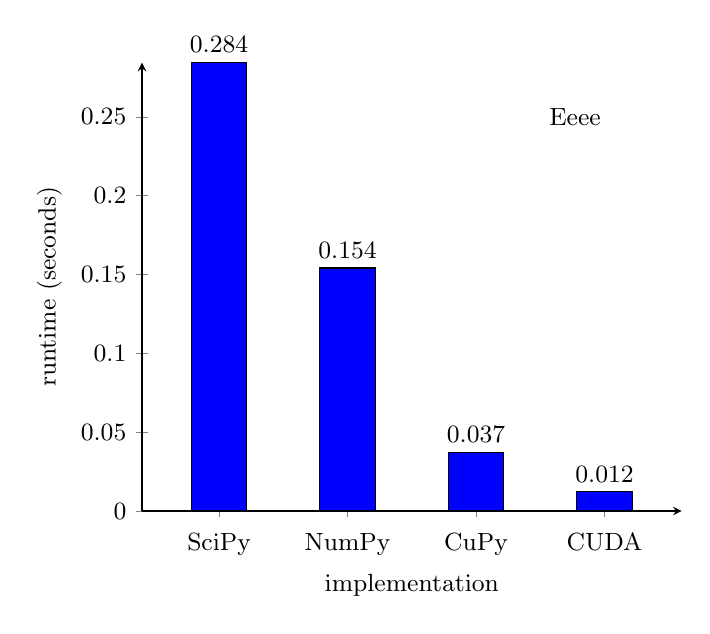
\begin{tikzpicture}[font=\small]

    \pgfplotsset{
      compat=newest,
      xlabel near ticks,
      ylabel near ticks
    }

    \pgfplotsset{compat=1.11,
        /pgfplots/ybar legend/.style={
        /pgfplots/legend image code/.code={%
           \draw[##1,/tikz/.cd,yshift=-0.25em]
            (0cm,0cm) rectangle (3pt,0.8em);},
       },
    }

    \node at(5.5,5)(title){Eeee};
 
\begin{axis} [
  ylabel={runtime (seconds)},
  xlabel={implementation},
  ybar,
  bar width=20pt,
  ymin=0,
  xtick=data,
  axis x line=bottom,
  axis y line=left,
  enlarge x limits=0.2,
  symbolic x coords={SciPy, NumPy, CuPy, CUDA},
  xticklabel style={anchor=base, yshift=-\baselineskip},
  /pgf/number format/.cd,fixed,precision=3,
  nodes near coords={\small\pgfmathprintnumber{\pgfplotspointmeta}},
  legend style={anchor=west},
]

\addplot[fill=blue] coordinates {
    (SciPy, 0.2843504619598389)
    (NumPy, 0.15413585186004639)
    (CuPy, 0.037178173065185546)
    (CUDA, 0.012188527584075928)
};

\end{axis}
 
\end{tikzpicture}
\caption{Runtime in seconds averaged over 100 function calls where len(k) = len(r) = 40,000,000}
%\end{center}
\end{figure}

\begin{figure}[ht!]\label{figure:poisson_logpmf_performance_detailed}
\hspace*{3cm}
%\begin{center}
  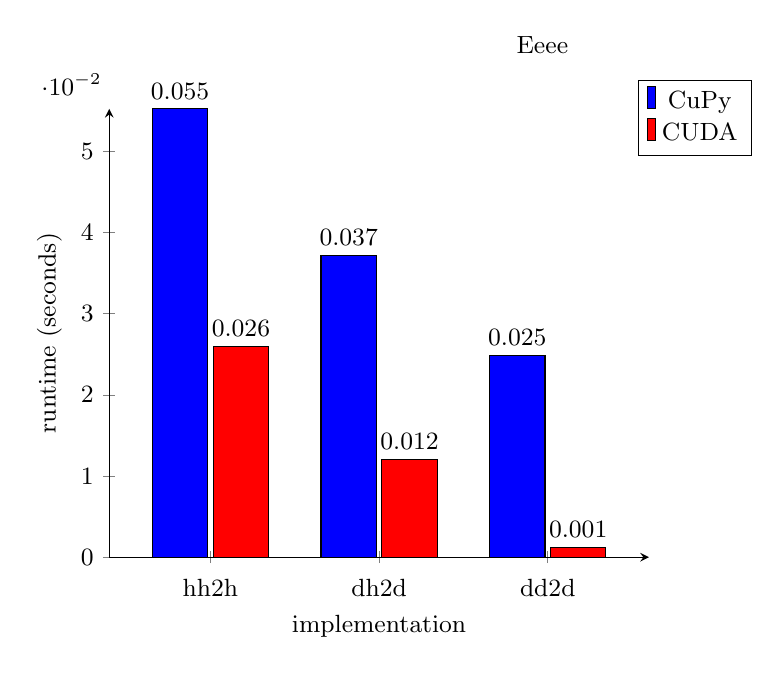
\begin{tikzpicture}[font=\small]

    \pgfplotsset{
      compat=newest,
      xlabel near ticks,
      ylabel near ticks
    }

    \pgfplotsset{compat=1.11,
        /pgfplots/ybar legend/.style={
        /pgfplots/legend image code/.code={%
           \draw[##1,/tikz/.cd,yshift=-0.25em]
            (0cm,0cm) rectangle (3pt,0.8em);},
       },
    }

    \node at(5.5,6.5)(title){Eeee};
 
\begin{axis} [
  ylabel={runtime (seconds)},
  xlabel={implementation},
  ybar,
  bar width=20pt,
  ymin=0,
  xtick=data,
  axis x line=bottom,
  axis y line=left,
  enlarge x limits=0.3,
  symbolic x coords={hh2h, dh2d, dd2d},
  xticklabel style={anchor=base, yshift=-\baselineskip},
  /pgf/number format/.cd,fixed,precision=3,
  nodes near coords={\small\pgfmathprintnumber{\pgfplotspointmeta}},
  every y tick scale label/.style={at={(yticklabel cs:1.1)},anchor=north},
  legend style={anchor=west},
]

\addplot[fill=blue] coordinates {
    (hh2h, 0.05520418882369995)
    (dh2d, 0.03713878393173218)
    (dd2d, 0.024829792976379394)
};

\addplot[fill=red] coordinates {
    (hh2h, 0.025965402126312254)
    (dh2d, 0.012055506706237793)
    (dd2d, 0.0012424540519714354)
};

\legend{CuPy, CUDA}
\end{axis}
 
\end{tikzpicture}
\caption{Runtime in seconds averaged over 100 function calls where len(k) = len(r) = 40,000,000}
%\end{center}
\end{figure}

\begin{figure}[ht!]\label{figure:experimental_poisson_logpmf_performance}
\hspace*{3cm}
%\begin{center}
  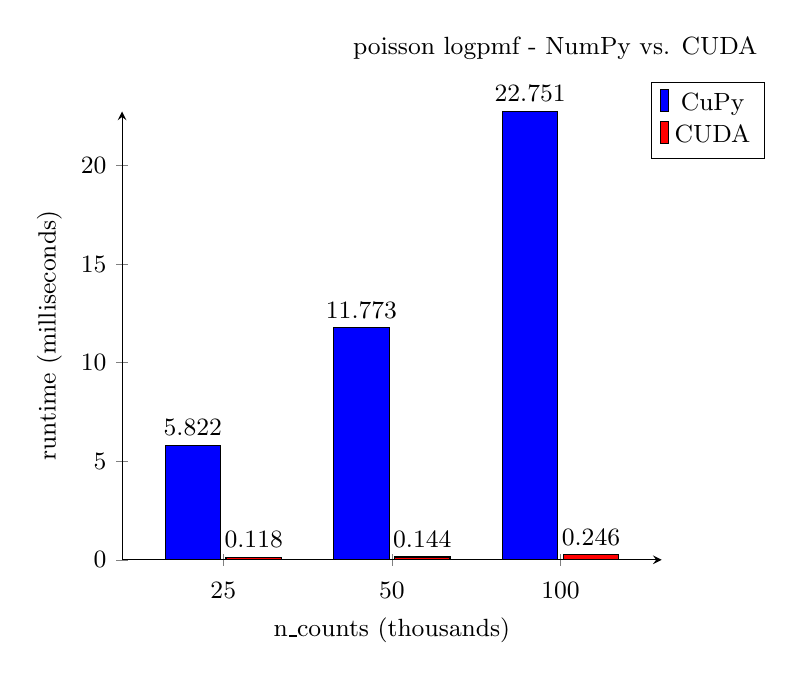
\begin{tikzpicture}[font=\small]

    \pgfplotsset{
      compat=newest,
      xlabel near ticks,
      ylabel near ticks
    }

    \pgfplotsset{compat=1.11,
        /pgfplots/ybar legend/.style={
        /pgfplots/legend image code/.code={%
           \draw[##1,/tikz/.cd,yshift=-0.25em]
            (0cm,0cm) rectangle (3pt,0.8em);},
       },
    }

    \node at(5.5,6.5)(title){poisson logpmf - NumPy vs. CUDA};
 
\begin{axis} [
  ylabel={runtime (milliseconds)},
  xlabel={n\_counts (thousands)},
  ybar,
  bar width=20pt,
  ymin=0,
  xtick=data,
  axis x line=bottom,
  axis y line=left,
  enlarge x limits=0.3,
  symbolic x coords={10, 25, 50, 100},
  xticklabel style={anchor=base, yshift=-\baselineskip},
  /pgf/number format/.cd,fixed,precision=3,
  nodes near coords={\small\pgfmathprintnumber{\pgfplotspointmeta}},
  every y tick scale label/.style={at={(yticklabel cs:1.1)},anchor=north},
  legend style={anchor=west},
]

\addplot[fill=blue] coordinates {
    (25, 5.82169)
    (50, 11.77253)
    (100, 22.75124)
};

\addplot[fill=red] coordinates {
    (25, 0.11837)
    (50, 0.14367)
    (100, 0.24571)
};

\legend{CuPy, CUDA}
\end{axis}
 
\end{tikzpicture}
\caption{Runtime in seconds averaged over 1000 function calls with n\_counts=50,000}
%\end{center}
\end{figure}

\subsubsection{Hey}

\begin{compactitem}
  \item
    49.2x speedup

  \item
    81.9x speedup

  \item
    92.6x speedup
\end{compactitem}

\begin{figure}[ht!]\label{figure:experimental_poisson_logpmf_performance_speedups}
\hspace*{3cm}
%\begin{center}
  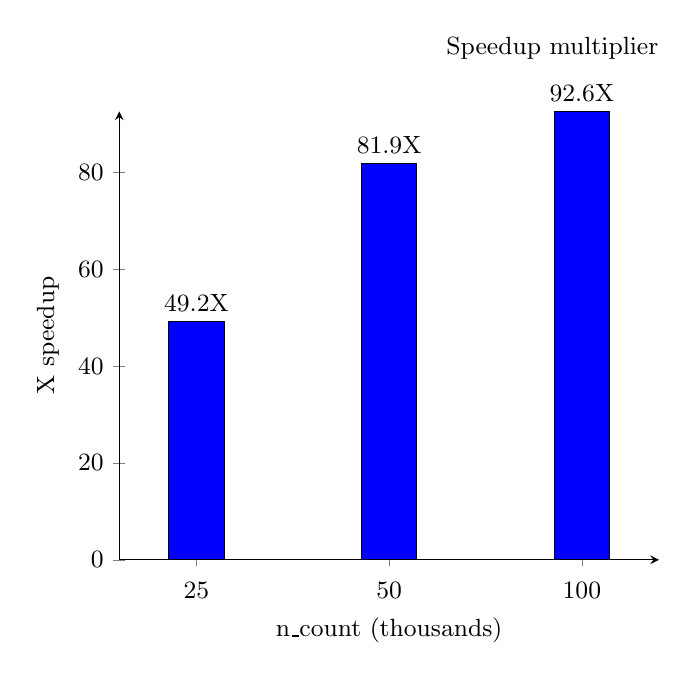
\begin{tikzpicture}[font=\small]

    \pgfplotsset{
      compat=newest,
      xlabel near ticks,
      ylabel near ticks
    }

    \pgfplotsset{compat=1.11,
        /pgfplots/ybar legend/.style={
        /pgfplots/legend image code/.code={%
           \draw[##1,/tikz/.cd,yshift=-0.25em]
            (0cm,0cm) rectangle (3pt,0.8em);},
       },
    }

    \node at(5.5,6.5)(title){Speedup multiplier};
 
\begin{axis} [
  ylabel={X speedup},
  xlabel={n\_count (thousands)},
  ybar,
  bar width=20pt,
  ymin=0,
  xtick=data,
  axis x line=bottom,
  axis y line=left,
  enlarge x limits=0.2,
  symbolic x coords={25, 50, 100},
  xticklabel style={anchor=base, yshift=-\baselineskip},
  /pgf/number format/.cd,fixed,precision=3,
  nodes near coords={\small\pgfmathprintnumber{\pgfplotspointmeta}X},
  legend style={anchor=west},
]

\addplot[fill=blue] coordinates {
    (25, 49.2)
    (50, 81.9)
    (100, 92.6)
};

\end{axis}
 
\end{tikzpicture}
\caption{Eeee}
%\end{center}
\end{figure}
